\acresetall
\chapter{Artificial Intelligence}\label{ch:ml_intro}

\section{Overview}
\emph{Intelligence} as a concept has been a topic of exhaustive research in fields such as neurology, philosophy, neuroscience, neurobiology, and data science, among others. The Oxford dictionary defines intelligence as \emph{"the ability to acquire and apply knowledge and skills"} \cite{Oxforda}. The first part of this definition applies to what is known as "learning", which is according to the accepted definition of the term as well \cite{Oxford}, and that supports, from the etymology, the importance of the process of learning on intelligence.\\

Jeff Hawkins, a dedicated neuroscientist and author, has approached the subject from the engineering and medical flanks, analyzing the structure of the brain and having the perspective of the possibilities of replicating artificially the most sophisticated type of intelligence found on Earth: the human. In his book \emph{On Intelligence} \cite{HawkinsJeff2004}, he captures his findings after inspecting the brain cortex and making a parallel between humans and machines. According to Hawkins, \emph{"it is the ability to make predictions about the future that is the crux of intelligence"}, and these predictions are based on the experiences from which the intelligent being has learned, making decisions that lead it to the best possible known result. In order to create artificially a so-called \emph{intelligent agent}, scientist have put extensive efforts first on trying to replicate the known human intelligence \cite{Brooks1991}\cite{Reed2007}\cite{Hawkins}, taking the approach of generating a machine that is human-like and that behaves like one, being able to observe its surroundings, learn from stimulus that comes from the real world, adapt to changes, plan accordingly to foreseeable process (therefore, make predictions), make decisions and act appropriately. These are the characteristics that Mitola \cite{Mitola1999} described in the cognition cycle for \ac{CR}, which can be applied to any intelligent agent and, consequently, motivate the further research of \ac{AI}.\\

\ac{AI}, however, encircles a variety of disciplines that are in themselves a complete course of research, as it can be seen in Fig~\ref{fig:ai}. This work focuses only on the top branch: \ac{ML}. However, given the slight differences regarding implementation, a separate section will be dedicated solely to \ac{DL}.

\begin{figure}[htb]
    \centering
      \includestandalone[width=\textwidth]{figures/ai_tree}
      \caption{Artificial Intelligence}
      \label{fig:ai}
\end{figure}

\section{Machine Learning}
\ac{ML} encloses the process of taking a data set that represents any phenomena and learning from it. Any type of being that is capable of learning from previous experiences is showing a kind of intelligence, as it interiorizes the stimulus/data and reacts accordingly when it presents itself again. The vast majority of living beings have this capacity, being the humans who have the lead on its effectiveness. Identifying objects, speaking languages, and reacting to any sensorial stimulus is a result of a successful learning process. \\

Generally speaking, learning from data is done when there is no analytic solution to an encountered situation, but there is enough data to adapt to it, generating an empirical solution to a problem that cannot be mathematically a-priori described, but that follows a specific pattern\cite{Yaser}. Just as humans do, the idea of \ac{ML} is to generate intelligent agents computationally - teach computers to learn. The idea is as follows: a \ac{ML} algorithm is given a set of data from which it can extract specific information that tells it the specifics about the data. With enough information, the computer is able to make predictions about other data in a different point in time if this data presents the same characteristics.

Although there is no specific mathematical representation of the specific problem to solve, many \ac{ML} algorithms rely heavily on mathematical definitions and optimization theory. Further information regarding \ac{ML} algorithms can be found in section~\ref{ch:ml_algs}. The versatility provided by the fact of not needing to pin down the specific analytic description of the problem is what has allowed this methodology to be applied in several fields of knowledge, being nowadays used to solve problems in areas such as financial forecasting\cite{Bose2001}, medical diagnosis\cite{Kononenko2001}, entertainment\cite{Bennett2007} and communications systems (such as this thesis), among others. Examples of everyday problems that are suitable for \ac{ML} implementation are:

\begin{itemize}
    \item Ranking links and clicks for a better web search engine and advertisements.
    \item Custom user recommendations based on purchases/rents/views.
    \item Prediction of markets and stock exchange.
    \item Dating sites with a reevaluation of algorithms based on successful matches.
    \item Financial fraud detection.
    \item Supply chain optimization
    \item Biotechnology research acceleration by sequencing and screening of DNA and protein/compound structures.
    \item National security based on enormous surveillance data.
\end{itemize}

\subsection{The learning problem}
Learning from data is definitely a hot topic, which can be seen from the increasing amount of research and application that has been handed over this theory and methodology. Additionally, it is noticeable how the term has been capturing the mainstream interest and is somewhat heard-of, as it can be seen in the Fig.~\ref{fig:ml_trend}, where this trend over the past few years is clear. At this point, it is preeminent to clarify what is the purpose of \ac{ML}, and when it plays an important role. Although \ac{ML} has shown to perform outstandingly into solving many problems, it is not intended to move aside the many and well-designed analytic solutions for many of the scientific existing problems, but to come in handy when that analytic solution does not describe completely the problem, or does not exist. In his book \cite{Yaser}, Prof. Yaser nicely states that although many problems can be solved effectively using a learning approach or an analytic approach, the point of learning is not to compare itself and overcome the performance over the mathematical description of existing problems, but to be a complementary tool for scientist in their eagerness to solve complex problems without being stuck when facing the lack of a complete description of it.

\begin{figure}[htb]
    \centering
      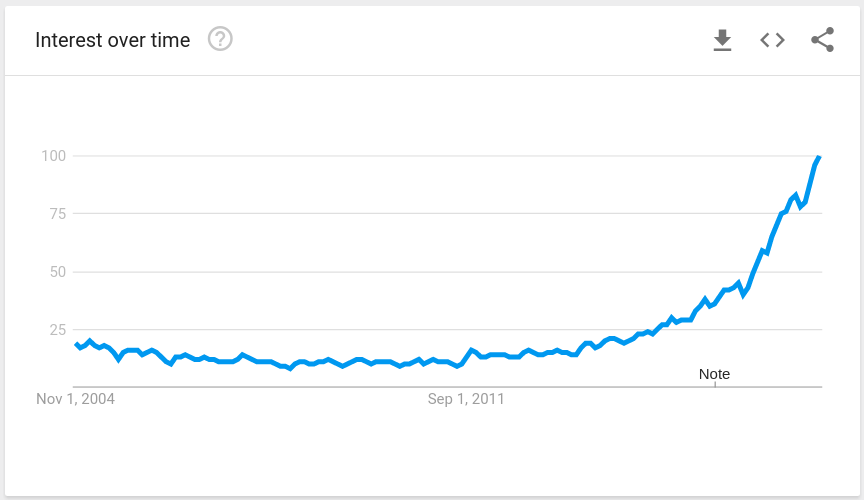
\includegraphics[width=0.6\textwidth]{figures/ml_trend.png}
      \caption{'Machine learning' Google search trend \cite{GoogleInc.2017}}
      \label{fig:ml_trend}
\end{figure}

The learning problem is summarized in Fig~\ref{fig:learning_problem} and follows the theoretical description provided at \cite{Yaser}. The learning algorithm \( \mathcal{A} \) receives data of any form, and its sole purpose is to identify mechanisms that describe that dataset \( \mathcal{D} \) closely. This dataset is defined as input-output samples for the supervised learning, input-weights samples for reinforcement learning and only inputs for the unsupervised learning. Further information regarding supervised, reinforcement and unsupervised learning can be found in section~\ref{ch:learning_types}. For the sake of the explanation, let us take the supervised learning case, where the dataset  \( \mathcal{D} \) includes samples of the form \((\mathbf{x}_1, y_1),\cdots , (\mathbf{x}_N, y_N) \), where \(x\) is the input that belongs to the input space \( \mathcal{X} \), \(y\) is the corresponding output such that \(y_n = f(x_n)\), and belongs to the output space \( \mathcal{Y}\). Now, the learning algorithm \( \mathcal{A} \) needs to find that function \(f(x)\). For this, it employs a hypothesis set \( \mathcal{H} \), which are the mathematical representations that the algorithm uses as tools to accomplish its purpose. From \( \mathcal{H} \) the algorithm takes one hypothesis \( g:\mathcal{ X \rightarrow Y} \) that approximates \(f\). After a \(g\) has been selected, the process estimates how alike the outputs from \(g(x)\) are to \(f(x)\), and feedbacks an error measure \(E(g,f)\). This process is repeated iteratively until a hypothesis produces an acceptable minimum error. \\

\begin{figure}[htb]
    \centering
      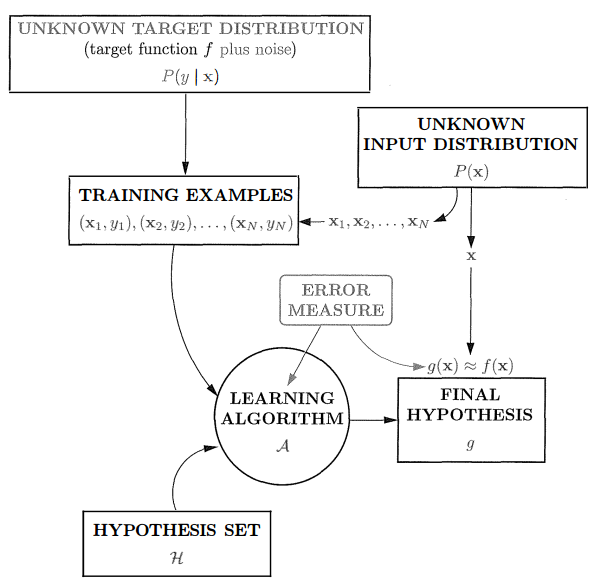
\includegraphics[width=0.6\textwidth]{figures/learning_problem.png}
      \caption{The learning problem \cite{Yaser}}
      \label{fig:learning_problem}
\end{figure}

Now, it is imperative to determine quantitatively what exactly \emph{acceptable} means. Different applications can have different tolerances to error, and this affects directly the hypothesis \( g \) that is chosen at the end of the learning process. This means that this is an end-user parameter that has to be set as a requirement for the whole system.

After taking different samples from \( \mathcal{X} \), and reducing the error, we should take into account the samples that \emph{we did not take}, meaning the samples that are not in our input set, and that probably behave similarly to the \( \mathcal{X} \) set - i.e. we should be able to identify similar samples in order to be able to predict. Therefore, a probability distribution is added to both the input samples and the final hypothesis in order to infer from \( \mathcal{D} \) the behavior of samples that are not in \( \mathcal{D} \). Let us assume a binary classification problem, where \( \mathcal{D} \) contains two classes, A and B, in a possibly infinite number. From a random sample pick the probability that the input sample is of the A type will be denoted as \(\mu\) and, consequently, the probability that the input sample is of the B type is 1 - \(\mu\). The value of \(\mu\) is unknown and will continue to be unknown in the process. From a random pick of N samples from \( \mathcal{D} \), there is a proportion of \(\nu\) samples of the A-type, and we intend to determine how \(\nu\) relates to \(\mu\). In statistical jargon, we want to determine how our sample relates to the whole population. \\

From any point of view, the larger the sample that contributes to \(\nu\), the closer the relation it has with \(\mu\), but this relationship can be quantified using the \emph{Hoeffding Inequality} \cite{Hoeffding1963}, which states that for any sample size \(N\),

\begin{equation}
  \mathbb{P}[|\nu -\mu|>\epsilon ]\leq 2e^{-2\epsilon^{2}N} \quad \text{for any}\quad \epsilon>0
\end{equation}

Where \(\mathbb{P}[\cdot]\) denotes the probability with respect to the chosen sample, and \(\epsilon\) can be any positive value chosen by the data scientist, and represents the tolerance of error. This inequality says, simply put, that as the sample size \(N\) grows, it is \emph{exponentially unlikely} that the realization \(\nu\) deviates from \(\mu\) by more than the tolerance \(\epsilon\). It can be clearly seen that only the size of the sample \(N\) affects this bound. Consequently, to achieve a small tolerance \(\epsilon\), a large \(N\) has to be used.\\

Additionally, it is important to take into account the intrinsic noise of the systems, which can come from the nature of the input samples, i.e the samples are not product of a deterministic system, or are immersed into some stochastic variation that can be modeled by noise, and that implies that by having the same input into the system \emph{it is probable} to get a different output. This entails a change in the labels of the model. That is, instead of having \(y = f(x)\), we take \(y\) as a random variable resulting from a probability distribution \(P(y|x)\). Accordingly, the input data points are therefore generated by the joint distribution \(P(x,y) = P(x)P(y|x)\). With this description of the model, our target function (what \(\mathcal{A}\) wants to learn) becomes \(P(y|x)\), while \(P(x)\) quantifies the importance of the input \(x\) in our learning accuracy.

\subsection{Types of learning}\label{ch:learning_types}

There are three types of learning: supervised-, unsupervised-, and reinforcement learning. Each of them has specific characteristics, which are explained in the following subsections.

\subsubsection{Supervised learning}
Is the type of learning where, in addition to the input dataset, the explicit correct outputs for those given inputs are given to the \ac{ML} algorithm for training. There are two types of supervised learning:
\begin{itemize}
    \item \textbf{Classification:} consists in predicting a \emph{class label} from a determined set of choices. If the number of choices is two, the model corresponds to a \emph{binary classification}. As it has only two options, it is suitable for the problems whose expected answer is of the form "yes/no", "present/not present", "valid/invalid". For a greater number of classes, the model corresponds to a \emph{multiclass classification}. \cite{Andreas} Provides a simple list of examples of classification:
        \begin{itemize}
            \item Determining whether an email is spam or not constitutes a binary classification problem.
            \item Identifying the zipcode from handwritten digits on an envelope is a multiclass classification problem.
            \item Determine whether a tumor is benign based on size and shape data constitutes a binary classification problem
        \end{itemize}
    \item \textbf{Regression:} consists in predicting a continuous behavior, such as a trend, or a floating-number, and it is this continuity what sets it apart from the classification models. Examples of regression \cite{Andreas} are:
        \begin{itemize}
            \item Predict the value of the stock market
            \item Determine the expected amount of crops yield from a plantation based on data such as previous yields, weather history, etc.
        \end{itemize}
\end{itemize}

\subsubsection{Unsupervised learning}
Unlike supervised learning, in unsupervised learning the algorithms are feed with data but not with the expected outputs, which make this type of learning suitable for solving problems to which the output is unknown. The model is then in charge of extracting knowledge from the input data all by itself, without no further instructions. There are mainly two types of unsupervised learning that can be found in the literature \cite{Andreas}, which are the \emph{unsupervised transformations} and \emph{clustering}.

\begin{itemize}
    \item \textbf{Unsupervised transformations:} consists in creating new representations of the input data, so that it becomes easier to understand and/or to use than the original data. This functionality is used, for example, to reduce the dimensionality of data that consists of several features. In such a situation, the model transforms the data into a representation that summarizes the input with fewer features. Another important use of this type of models is finding the overall representation of the input data, such as the topic of a full text, or the sentiment in a short comment.
    \item \textbf{Clustering:} this kind of models collects the data into determinate groups that share similar characteristics. This is used, for example, to generate suggestions based on previous purchases/views, or to group pictures from a directory with several images to the ones that contain certain people (and suggest tagging the names on them).
\end{itemize}

As the models do not know beforehand what type of information they are intended to learn, one of the tasks of the data scientist is to assess that the model is indeed learning something useful. This creates the opportunity for this sort of models to be used for the same data scientist to help them identify certain characteristics of the data that were not obvious for the \emph{human-eye}, and certainly get a different perspective of the data from the \ac{ML} model point-of-view.

\subsubsection{Reinforcement learning}
This type of learning has a different approach to the previous two descriptions. Just like unsupervised learning, the model does not receive the expected outputs for the inputs it is given but, in contrast, it receives some \emph{possible} output along with a weight that states how good of an output it is. The idea behind this is that the model is then penalized when it provides a solution that is not according to the possible output and is rewarded when it is. Then, the model uses these penalizations and rewards to adjust the type of outputs it generates, and so it eventually learns the correct behavior for the situations it has been immersed into. This type of learning is similar to the way humans learn, in ways such as being penalized with pain when taking a sip of very hot coffee, or rewarded when winning a game of chess.\\

In that same manner, reinforcement learning comes in handy in teaching an intelligent agent how to play a game, where it is presented to a plethora of options (which makes it difficult to be modeled as a supervised learning problem) and has to choose the one that brings it near to victory. The most recent example is AlphaGo \cite{Fu2017}, an intelligent agent capable of winning against the World Champion in a Go game. A similar approach has been followed by IBM with the Deep Blue chess-playing machine \cite{Hsu1999}.

\subsection{Training \& testing Models}
Training and testing are concepts that, when applied to learning algorithms, are not far away from the definitions that are used in common language when applied to humans. In general, \emph{training} a learning model consists of supplying it with enough data from which it can extract information and create generalizations, and testing consists of providing similar data to the model and identify if the generalizations apply. "Generalization" in this context means inferences, decisions or choices that the model makes on data it has never seen before based solely on the data it has learned from, and clearly, the goal of \ac{ML} is to have models that are able to generalize as accurately as possible. However, all learning scenarios depend on data, and this data, being as extensive as it can be, does not contain all the information that describes its surroundings completely. Therefore, the question arises: how can it be determined if the model can indeed learn to generalize from data?\\

The way to tackle this problem is separating the data into two: A portion of it to be used for training, and the rest of it to be used for validation/testing. Being the training set and testing set generated from the same whole dataset, it is expected that they share enough characteristics for the model to perform well at generalizing. However, there are cases when the model is too complex, and instead of learning to generalize it \emph{memorizes} the training set, and then performs poorly on the training set and on any unknown data. This phenomenon is known as \emph{overfitting} because the model is fit intimately to the training set as is not able to generalize on new data. That being said, one might think that creating the simplest learning model will never end up in overfitting, which is absolutely true. However, in such cases, the model might not be able to even capture the descriptive characteristics of the data, and ends up being incapable of learning from it. This phenomenon is known as \emph{underfitting}. Fig~\ref{fig:model_complexity} relates the complexity of the model with its capability of generalizing from new data.

\begin{figure}[!htb]
    \centering
      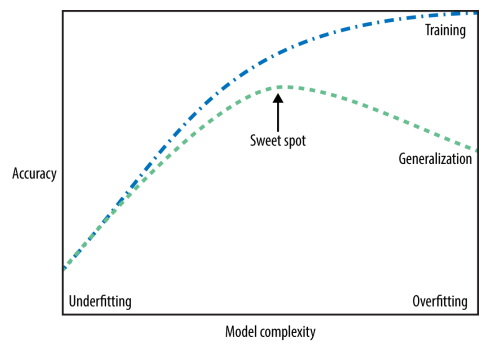
\includegraphics[width=0.6\textwidth]{figures/model_complexity}
      \caption{Model complexity vs. Training and test accuracy \cite{Andreas}}
      \label{fig:model_complexity}
\end{figure}

Therefore, it is clear that the objective model is not too simple or too complex, but somewhere in between; what \cite{Andreas} legitimately calls "the sweet spot", where the model has learnt as much as it can from the provided data, and is still able to create accurate inferences from unknown samples, ergo make predictions.


\subsection{Influence of dataset size in the learning process}\label{ch:size}
It has been constantly repeated that having data is paramount, but "how much data is required?" is a question that will always be asked, and that, unfortunately, has no concrete answer. The logic answer to it is "use as much data as possible", which also follows the Hoeffding inequality presented earlier in this chapter. Data is limited and generally comes along with the description of the problem itself. What this means is that, in data science, it is common for the learning problem to be stated as "The problem to solve is X, and the data available for it is Y" \cite{Yaser}. Asking for more data is, in most cases, impossible, and the data scientist has to work with what it has. However, the way the scientist extracts information from the data could be the lever that turns a failing model into a successful one.

Moreover, the model complexity is tied to the amount of information that the dataset holds; i.e. if the dataset has considerable variety within, the model can allow itself to grow in complexity without overfitting. This variety usually comes intrinsically with larger datasets, but the clarification has to be made: it is not the size of the dataset what directly yields to variety, meaning that duplicating samples won't help, as repeated data provides no increase on entropy.

\subsection{Data preprocessing}
Possibly the data that is measured or handed over to solve a problem does not provide much information \emph{as is}. However, after some careful treatment, that data might be transformed in the specific characteristics that allow an accurate generalization. The process of extracting specific \emph{features} that describe the information contained in the \emph{raw} dataset is called \emph{feature extraction}. It has been said earlier that unsupervised learning can be used for this purpose, using techniques such as \emph{Principal Component Analyzis (PCA)}, which retrives uncorrelated data and transforms the dataset component-wise in order to determine the information contribution of this component to the whole dataset. Other uses for unsupervised learning in data preprocessing are multiclass visualization, dimensionality reduction and generally finding a representation of the data that is more informative for later processing.\\

Additionally, feature extraction can be done manually, where the data scientist analyzes the data and produces a new dataset with a more representative description of it. This \emph{manual} method is also called \emph{feature engineering}, and was used by the \ac{CEL} in the DySpan spectrum challenge. Those extracted features are used in this work. A description of the implemented feature extraction process can be found in section~\ref{ch:features}.

Other type of preprocessing the data is \emph{scaling}, which comes in handy when samples of different orders of magnitude, belonging to different classes, are compared. This can be done, for example, by removing the mean of all the samples and scaling them to unit variance. Another way of scaling is setting a minimum and a maximum value, and fit all the features inside that range.

\subsection{Model Evaluation}
There are multiple ways to evaluate the performance of \ac{ML} algorithms, and they are helpful to determine if the model is generalizing from data satisfactorily. In this work, we focus on multiclass classification, and one of the most thorough tools for model evaluation is the confusion matrix. When a confusion matrix is calculated for a multiclass classification problem, a square matrix with dimensions equal to the number of classes is generated. Fig~\ref{fig:conf_matrix} shows the confusion matrix configuration for a binary classification, where the classes are "positive" and "negative". Each cell of the matrix contains the number of samples from the testing set that was classified to that specific class. This means that the diagonal of the matrix states the number of correctly classified elements.

\begin{figure}[htb]
    \centering
      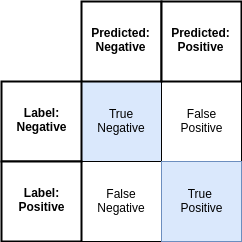
\includegraphics[width=0.4\textwidth]{figures/cm}
      \caption{Confusion Matrix}
      \label{fig:conf_matrix}
\end{figure}

Some applications have to regard specifically the type of misclassification that could happen in order to focus efforts into mitigating it. Prof. Yaser \cite{Yaser} exemplifies this with a fraudulent credit card transaction. If a fraudulent transaction is not happening, meaning that the rightful owner of the credit card is make use of the services he/she is entitled to, but the transaction is labeled as fraudulent, this has little negative consequences when compared with the situation in which a fraudulent transaction is indeed happening but is labeled as an honest one.

In this work, misclassification affects equaly the final output regardless of its type.
\subsection{\ac{ML} algorithms}\label{ch:ml_algs}
\subsubsection{K-nearest Neighbors}
This is one of the simplest \ac{ML} algorithms, and consists solely of making decisions based on the characteristics of the points that surround the point under test, i.e. the "nearest neighbors". It can be used for both supervised and unsupervised classification as well as for regression. The distance with which the "nearest" point is determined can be any metric measure such as:
\begin{itemize}
    \item Euclidian distance between any two points \( \sqrt{\sum (x - y)^2} \)
    \item Manhattan distance \( \sum {|x - y|} \)
    \item Chebyshev distance \( max(|x - y|) \)
    \item Minkowski distance \( \sum(|x - y|^p)^{1/p} \)
\end{itemize}
among others.

This algorithm is commonly called \emph{non-generalizing} because it remembers the location of its training data points and checks the proximity of its points to every other new data to predict. However, even though this procedure seems as "memorizing", this algorithm is not prone to overfitting and can lead to satisfactory results in datasets of various sizes, and because of its easiness to understand and apply, it is a good choice as a starting point for tackling a learning problem before applying more elaborated models. On very large datasets, or on datasets of very high dimensionality (several hundreds of classes) the amount of distances calculations escalates, which might lead to long prediction times.

\subsubsection{Decision trees}
This model is based on simple boolean-like bifurcations (if-then) that build a hierarchy tree that eventually leads to a decision, which makes it an uncomplicated model easy applicable in classification and regression. The concept can be easily explained with an example: assume that we have four common elements that can be found in a lab, such as an external monitor/screen, a laptop, an office chair and a USB stick. The classification of such can be as simple as it is shown in Fig~\ref{fig:dt_example}. In this example, the features are "has a screen?", "has wheels?" and "has a keyboard?". Clearly, this example model can be extended for further classification of lab elements.

\begin{figure}[!htb]
    \centering
      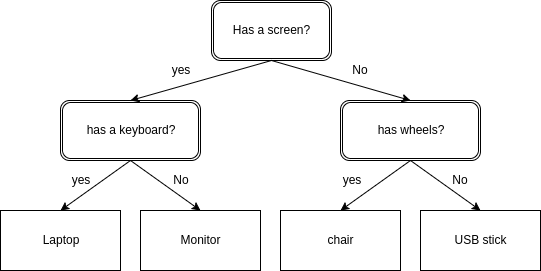
\includegraphics[width=0.7\textwidth]{figures/dt_example}
      \caption{Decision tree for classification of four lab elements}
      \label{fig:dt_example}
\end{figure}

The complexity of the model is given by the number of questions that have to be asked before reaching a final decision, i.e. the depth of the tree. With a long depth, the questions become more specific, and only a few samples are able to fit the tree, which leads to overfitting. In \ac{ML}, the tree is generated automatically, so a good way to avoid overfitting is stopping the tree from growing more than it should, in a process called \emph{pre-pruning}, or removing branches that provide little to no information after the tree has been created, which is called \emph{post-pruning}.

Given the nature of the decision tree, preprocessing the data (with methods such as scaling) does not influence its performance in terms of accuracy, because each feature is processed completely independent of the others. Because of this reason, this model is recommended when the features do not fall into a common range or have completely different characteristics (such as a mixture of discontinuous and continuous features).

\subsubsection{Support Vector Machines}
Support vector machines (SVM) are an extension of the linear models that serve as a base for classification systems, such as the perceptron, which is explained more in detail in section~\ref{ch:neural}. Basic linear models are not regarded in this work because they are not explicitly used in the implementation described in following chapters, and the specifics of the mathematic description for the linear models and \ac{SVM} models is extensive and out of the scope of this thesis. Prof. Yaser provides an extensive explanation of perceptrons and on its use for the learning process \cite{Yaser}. In summary, a linear model sets a classification boundary that separates different classes. \ac{SVM} extends this functionality by introducing the concept of \emph{hyperplanes}, which ensures an improved classification by maximizing the separation of points of different classes by the means of the hyperplanes. This classification boundaries are shown in Fig~\ref{fig:svm} for two different classes.

\begin{figure}[!htb]
    \centering
      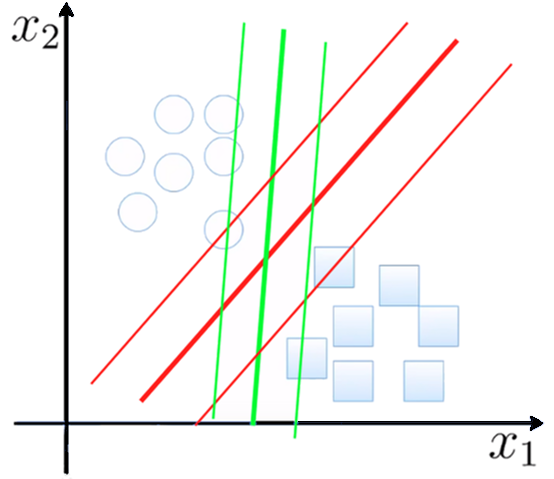
\includegraphics[width=0.5\textwidth]{figures/svm}
      \caption{\ac{SVM} - Hyperplanes separating two classes. Functional margin in red.}
      \label{fig:svm}
\end{figure}
The hyperplanes that generate the largest separation between training data points of different classes form a so-called \emph{functional margin}, which provides the smallest generalization error for the classifier. These models are said to have exceptionally good performance in high dimensional spaces, even when the number of classes is greater than the number of available samples \cite{SKLEARN}.

\section{Deep Learning}
Additionally, to the approach of learning from extracted features, deep learning is an approach based on learning data representations. This is a subgroup of \ac{ML} and was developed on top of a technique called Neural Networks, which is described briefly below. The term "Deep learning" was coined in 1986 by Rina Dechter \cite{Dechter}, in a proposed work to overcome a way to learn the maximum amount of information from techniques using backpropagation, making a parallel of learning and recording, and so when a so-called \emph{dead end} is encountered, the recorded information could guide iteratively to make new decisions.

\subsection{Neural Networks}\label{ch:neural}
Before getting deeper into the specifics of neural networks, it is precise to first define one small unit that is used to build the networks: the perceptron. A perceptron is a node that implements a very simple binomial linear classification. It maps the output based on an activation function applied to the input:

\begin{equation}
    f(x) =
    \begin{cases}
        1 \text{ if } w*x + b > 0\\
        0 \text{ otherwise}
    \end{cases}
\end{equation}

It can clearly be seen that the output of the perceptron is based on a linear equation of the form \(y=mx+b\), where \(w\) is a vector of weights, \(x\) is the input of the perceptron, and \(b\) is the bias. The weights set certain restrictions to the input data, and the bias determinates the decision threshold for a binary classification. Assuming that values higher than the threshold are set to a positive decision, and below the threshold to a negative decision, the mathematic representation is set as:

\begin{equation}
    \text{positive decision if } \sum_{i=1}^{d} w_i\cdot x_i > \text{bias}
\end{equation}
\begin{equation}
    \text{negative decision if } \sum_{i=1}^{d} w_i\cdot x_i < \text{bias}
\end{equation}

which can be represented in the following simplified form:
\begin{equation}
    \text{decision } h(x) = \text{sign}\left(  \left( \sum_{i=1}^{d} w_i\cdot x_i \right )+ b \right )
\end{equation}

A basic representation of a perceptron is shown in Fig~\ref{fig:perceptron}.

\begin{figure}[!htb]
    \centering
      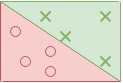
\includegraphics[width=0.4\textwidth]{figures/perceptron}
      \caption{Interconnection of perceptrons generating a simple neural network. \cite{Yaser}}
      \label{fig:perceptron}
\end{figure}

Perceptrons are also called \emph{neurons}, which are activated to specific types of input data. When more neurons are interconnected, each one with a different activation function (based on the weights and the bias), a neural network is created, which can then classify input data of higher complexity. An arbitrary amount of neurons can be added increasing as well the complexity of the network, but each of them classifies the data independently. Historically, the name \emph{neural network} is given because of the similarity of this behavior to the synapses of the neurons in a biological neural system. The book of professor Yaser \cite{Yaser} explains in further detail the perceptrons and the learning process using these units.

\begin{figure}[!htb]
    \centering
      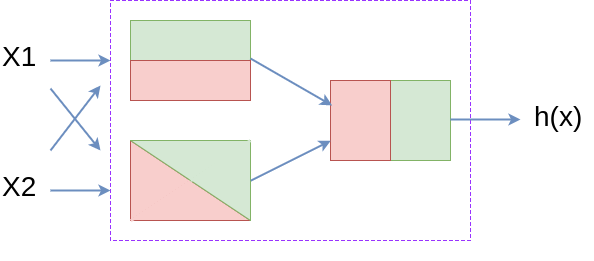
\includegraphics[width=0.8\textwidth]{figures/neuralnetwork}
      \caption{Basic structure of a neural network.}
      \label{fig:neuralnetwork}
\end{figure}

\subsection{Convolutional Neural Networks}

\ac{ConvNet} are a special type of neural networks that share their parameters across space, making them suitable for image classification. The main idea is as follows: assume we have an image depicted in blue in Fig~\ref{fig:convolutionalnetwork} as the input of this system, whose dimensions are (height, width, and depth). The height and width are the numbers of pixels that determine the size of the picture, and the depth is 3 for color pictures (RGB) and 1 for grayscale. When this picture is inserted into the \ac{ConvNet}, only a portion of it is regarded as a so called patch, shown in red.

\begin{figure}[t!]
    \centering
      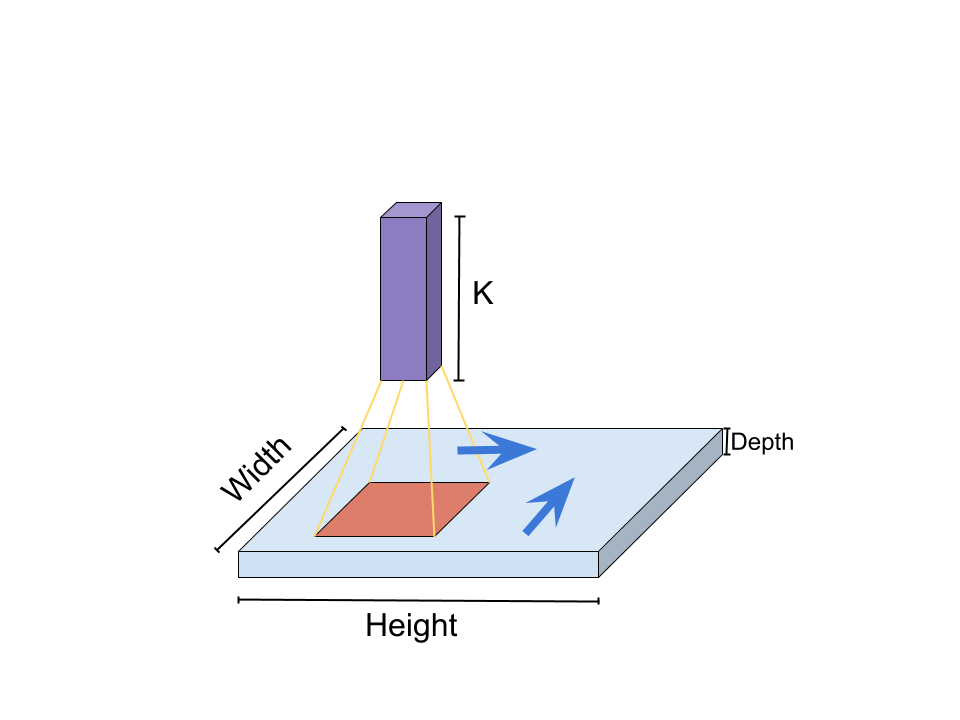
\includegraphics[width=\textwidth]{figures/convolutionalnetwork}
      \caption{Convolutional Network}
      \label{fig:convolutionalnetwork}
\end{figure}

This patch, also called kernel, is then swept along the picture with a given arbitrary stepsize, applying a neural network operation over it. As it is a smaller patch, each operation regards many fewer weights in comparison with the whole input, which is shared across space with the slide operation. As a result, a stack of convolutions is generated, representing a picture-like output, having not only a reduced height and width but an increased depth K that represents the non-linearities that describe the input, as if it increased the number of color channels that describe the input picture.\\

Generally, these convolutional layers are stacked together generating a pyramid, in a so-called sequential model, reducing the spatial dimensions of an input image (h,w), but increasing its depth. As a result, the depth corresponds to the \emph{semantic complexity} of the image representation, mapping the illustrative content of it. Inside of each layer, there is a number K of filters, in charge of picking different characteristics from the image, such as a specific shape or a determinate intensity value. The characteristic that the filter notices is not programmed, but learned by itself. This means that the network learns on its own what type of feature representation is going to learn and, consequently, which shape is going to activate it.


